This section shows the experimental results of the implementation proposed in Section~\ref{sec:method}. The framework is evaluated on the Rosario Dataset \cite{pire2019rosario}, a set of agricultural data captured by a weed removal robot. Later, an evaluation of the system in a soybean field is presented, using the same weed removal robot. The difference between the latter test and the evaluation on the Rosario Dataset is that new sensors are available, including measurements from a conventional GNSS.

\subsection{Rosario Dataset}
\label{sec:experiments_rosario_dataset}
The Rosario Dataset \cite{pire2019rosario} is a set of data captured by the sensors of a weed removal robot developed by the CIFASIS institute (CONICET-UNR) in Rosario, Argentina. It is composed of six sequences captured in a soybean field. The sequences contain stereo images of $672\times\SI{376}{\px}$ captured at \SI{15}{\hertz}, measurements from an IMU with a frequency of \SI{142}{\hertz} including gyroscope and accelerometer, wheel odometry obtained at \SI{10}{\hertz} and GNSS-RTK measurements at \SI{5}{\hertz}. The GNSS-RTK data are used as positional ground‐truth.

Since the Rosario Dataset does not have conventional GNSS measurements, we simulate noisy GNSS measurements by corrupting the ground-truth with zero-mean Gaussian noise, as in \cite{cioffi2020tightly}. We use isotropic Gaussian noise $\mathbf{n}_{p}\sim\mathcal{N}\left(\mathbf{0},\sigma_{p}^{2}\cdot\mathbf{I}\right)$, with a standard deviation $\sigma_{p} = \SI{0.5}{\meter}$. We selected this value from observing the covariance of the conventional GNSS used in the experiments in Section~\ref{sec:experiments_conventional_gps}. 

\begin{table}[!tp]
    \centering
    \caption{Mean and standard deviation (between parentheses) of the Absolute Trajectory Error (ATE) [\si{\metre}] for stereo-inertial ORB-SLAM3 \cite{campos2021orbslam3}, a loosely-coupled GNSS-stereo-inertial system \cite{qin2019general} and our tightly-coupled GNSS-stereo-inertial framework in the six sequences of the Rosario Dataset. Best results are in \bf{bold}.}
    
    \resizebox{\linewidth}{!} {
        \begin{tabular}{cccc}
        \hline
                    Sequence & Stereo-Inertial & GNSS-Stereo-Inertial & GNSS-Stereo-Inertial \\
                    & \cite{campos2021orbslam3} & \cite{qin2019general} & (Ours) \\
                    \hline
        01 &  0.90 (0.34)                  &
        1.44 (2.06) &
        \bf{0.86 (0.26)}                \\
        02 &  1.33 (0.75)                  &        \bf{0.90 (0.40)} &
        0.94 (0.56)                 \\
        03 &  1.12 (0.65)                  & 1.34 (1.91) & \bf{0.99 (0.56)}                \\
        04 & 1.09 (0.65)                   & 1.42 (1.20) &
        \bf{1.04 (0.60)}                \\
        05 &  0.89 (0.55)                  & 1.43 (1.91) & \bf{0.76 (0.38)}                \\
        06 & 2.48 (1.40)                   & 1.81 (0.87) &  \bf{1.23 (0.70)}     \\ \hline
        \end{tabular}
    }
    \label{tab:rosario_results}
\end{table}

We compared our GNSS-Stereo-Inertial implementation against Stereo-Inertial ORB-SLAM3 and a loosely-coupled GNSS-Stereo-Inertial system known as VINS-Fusion \cite{qin2019general}. VINS-Fusion was chosen because it is a state-of-the-art system that takes as input the same GNSS measurements as our system, i.e. latitude, longitude and altitude. Each system was run five times in each of the Rosario sequences, and Table~\ref{tab:rosario_results} presents the lowest ATE error of the five executions for each framework. ATE
has been computed after the estimated trajectories
were aligned with the ground-truth GNSS readings using Umeyama's method \cite{umeyama1991least}. The corresponding trajectories are presented in Figure~\ref{fig:trajectories_rosario}. %The biggest improvement can be seen in Sequence~06, a trajectory of approximately \SI{530}{\meter} in length.

\begin{figure*}[!htp]
  \centering
  \subfloat[Sequence 01\label{trajectories_sequence_01}]{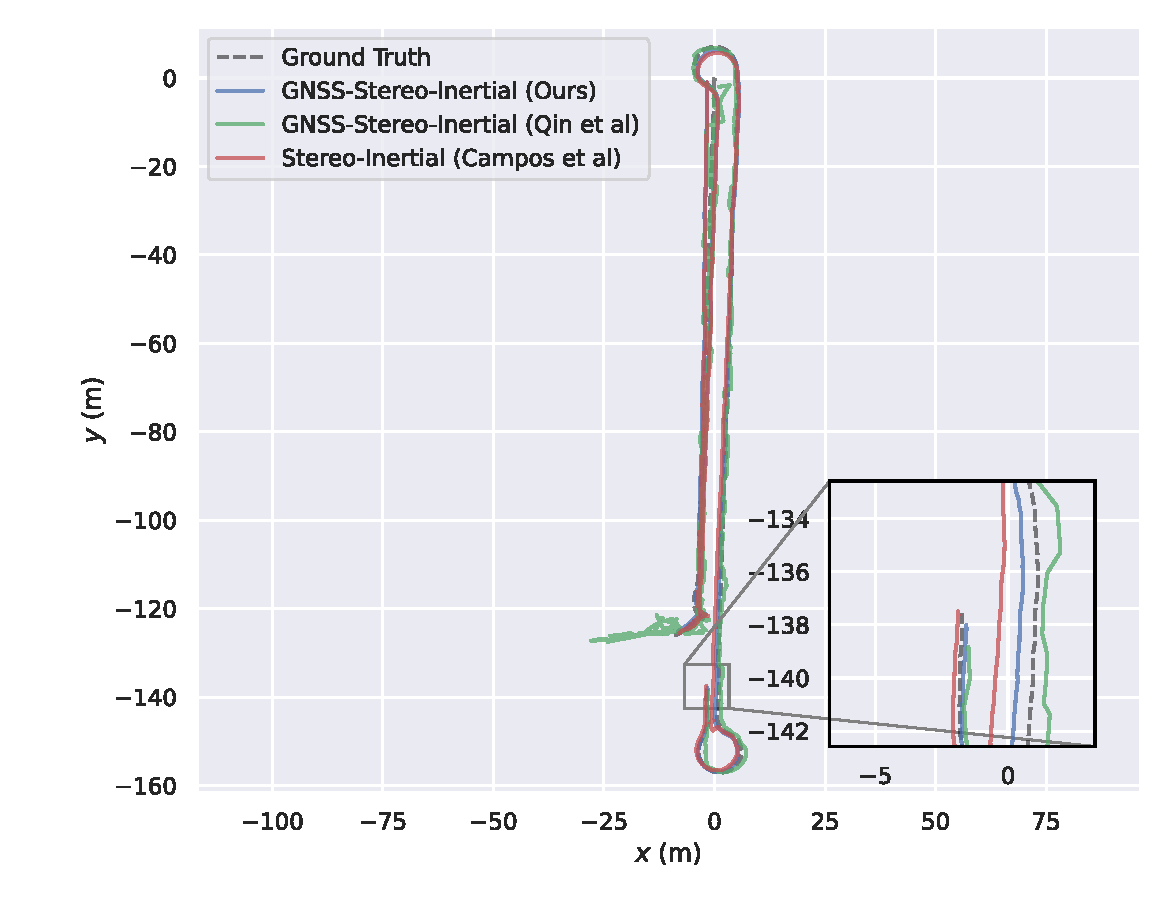
\includegraphics[width=0.42\textwidth]{images/seq01.pdf}}
  \hspace{1cm}
  \subfloat[Sequence 02\label{trajectories_sequence_02}]{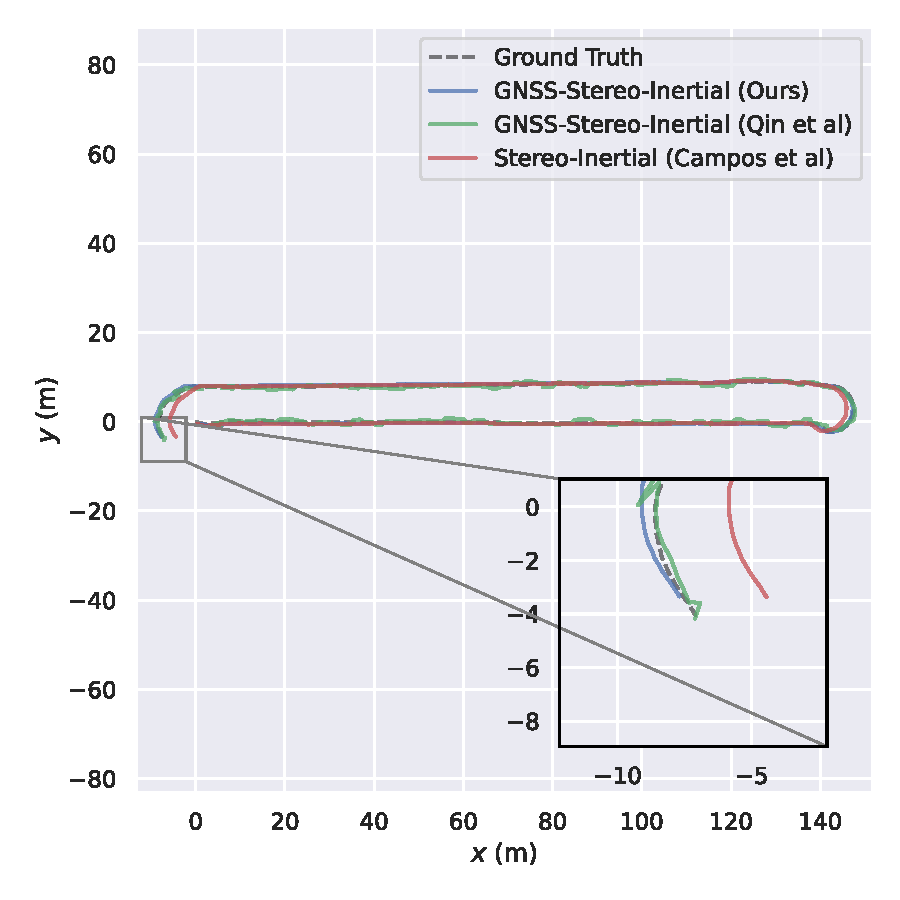
\includegraphics[width=0.42\textwidth]{images/seq02.pdf}\label{trajectories_sequence_02_int}}\\
  \subfloat[Sequence 03\label{trajectories_sequence_03}]{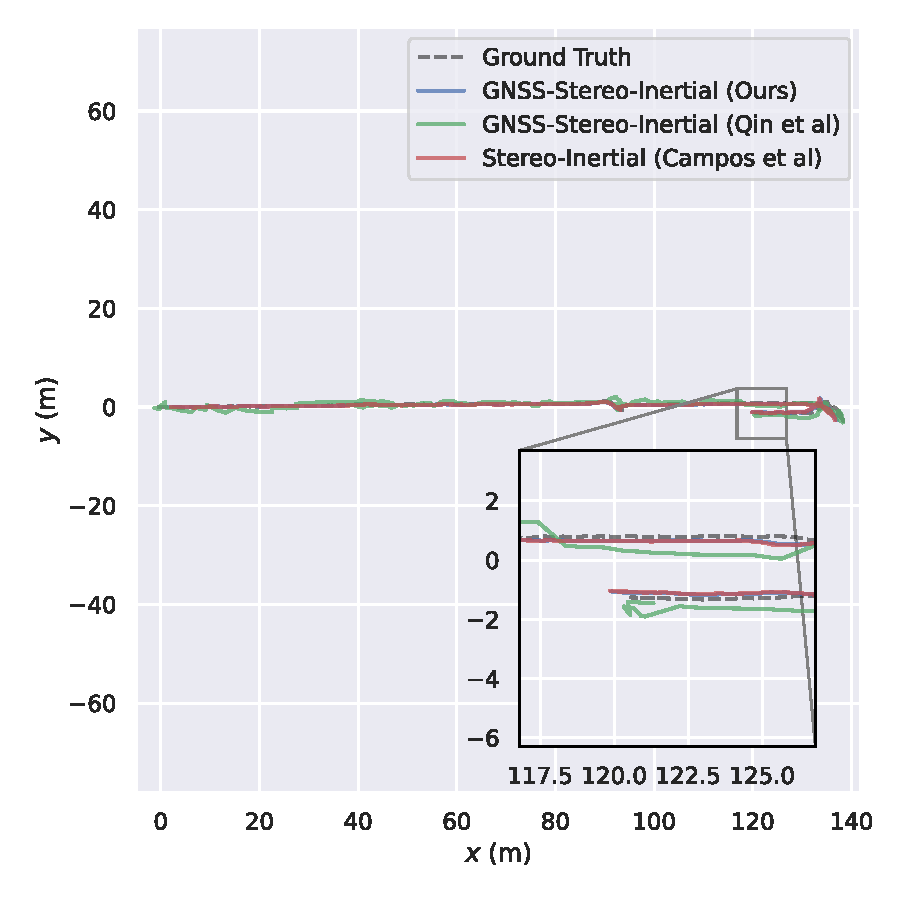
\includegraphics[width=0.42\textwidth]{images/seq03.pdf}}
  \hspace{1cm}
  \subfloat[Sequence 04\label{trajectories_sequence_04}]{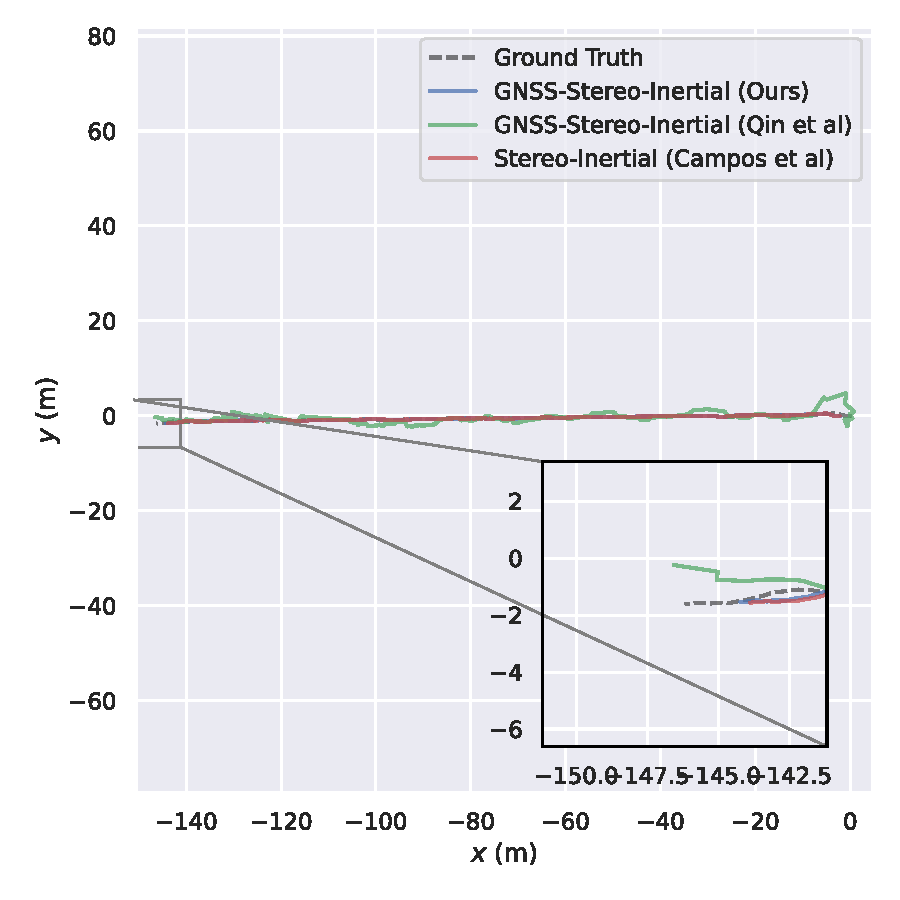
\includegraphics[width=0.42\textwidth]{images/seq04.pdf}}\\
  \subfloat[Sequence 05\label{trajectories_sequence_05}]{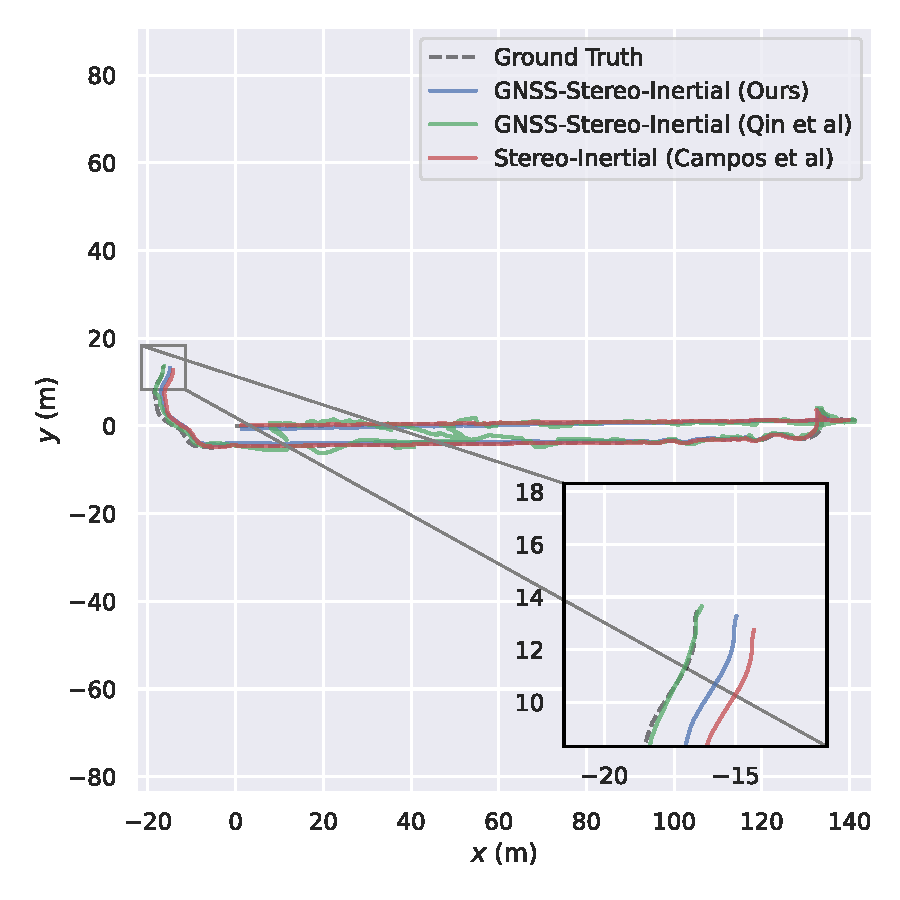
\includegraphics[width=0.42\textwidth]{images/seq05.pdf}}
  \hspace{1cm}
  \subfloat[Sequence 06\label{trajectories_sequence_06}]{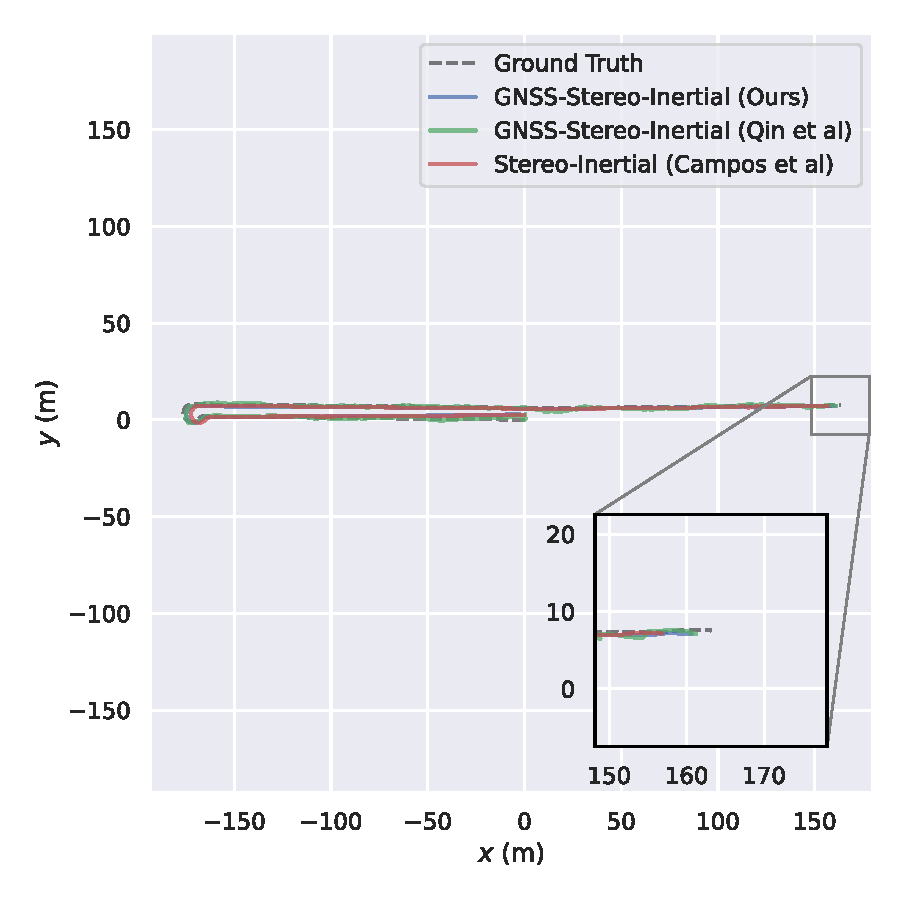
\includegraphics[width=0.42\textwidth]{images/seq06.pdf}}
  \caption{Results from Stereo-Inertial ORB-SLAM3 \cite{campos2021orbslam3}, a loosely-coupled GNSS-Stereo-Inertial system \cite{qin2019general} and our tightly-coupled GNSS-Stereo-Inertial system on the Rosario Dataset.}
  \label{fig:trajectories_rosario}
\end{figure*}

\subsection{Data with conventional GNSS in soybean fields}
\label{sec:experiments_conventional_gps}
In the experiments from the previous section, noisy GNSS measurements had to be simulated from GNSS-RTK ones, as the dataset does not contain conventional GNSS measurements. In this section we present an evaluation with conventional GNSS measurements. For this, we equipped our weed removal robot with such sensor and deployed it again in a soybean field. On board the robot there is a ZED stereo camera which captures images $\si{1280}\times\SI{720}{\px}$ at \SI{15}{\hertz}, an Emlid Reach GNSS operating at a frequency of \SI{5}{\hertz}, and an InvenSense MPU-9250 IMU set at \SI{200}{\hertz}. The covariance of the conventional GNSS measurements is offered by the driver of the GNSS receiver. In addition, there is an GNSS-RTK used as positional ground-truth. Figure~\ref{fig:robot} shows the robot configuration in the soybean field. We commanded the robot to record two data sequences. The corresponding GNSS-RTK trajectories are shown in Figure~\ref{fig:satellital} and images samples captured by the ZED camera can be seen in Figure~\ref{fig:image_samples}.

\begin{figure}[t]
    \centering
    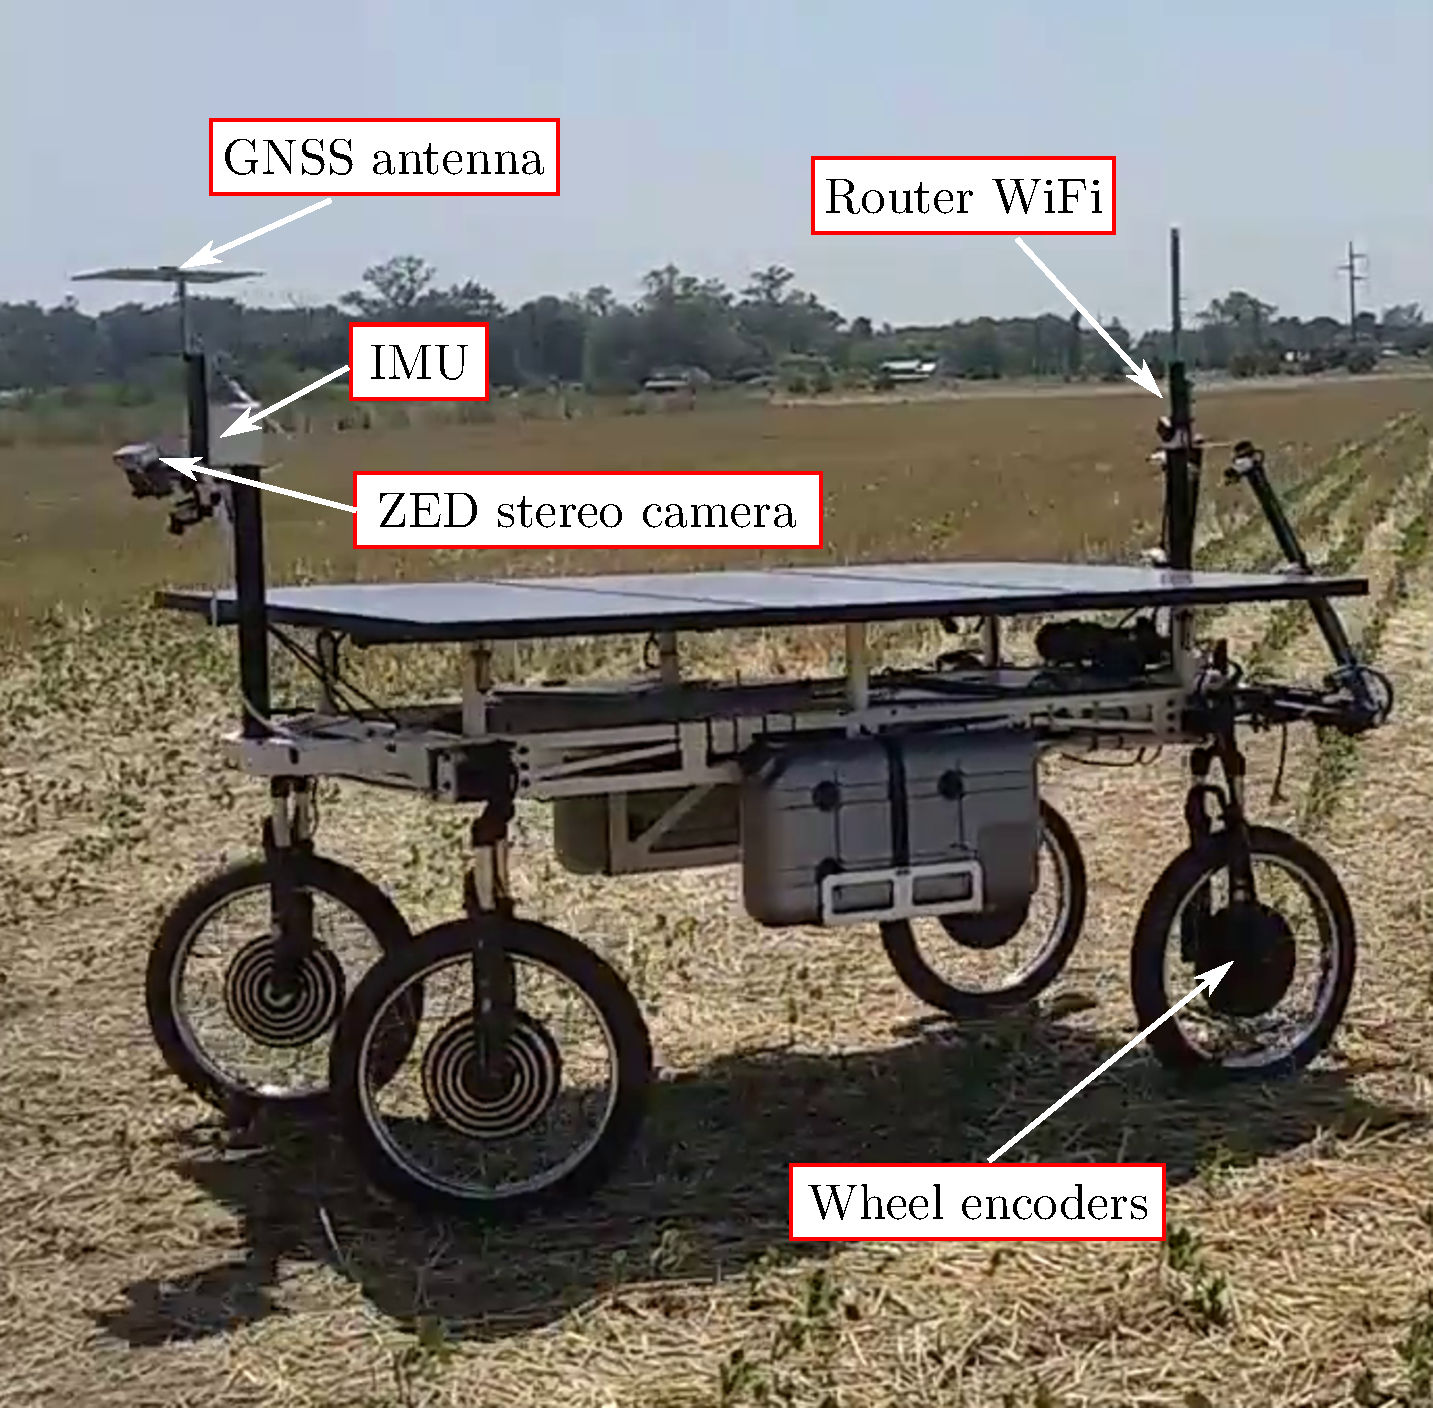
\includegraphics[width=\columnwidth]{images/robot_2022.pdf}
    \caption{Weed removal robot used in our in-house dataset in a soybean field.}
    \label{fig:robot}
\end{figure}

\begin{figure}[t]
    \centering
    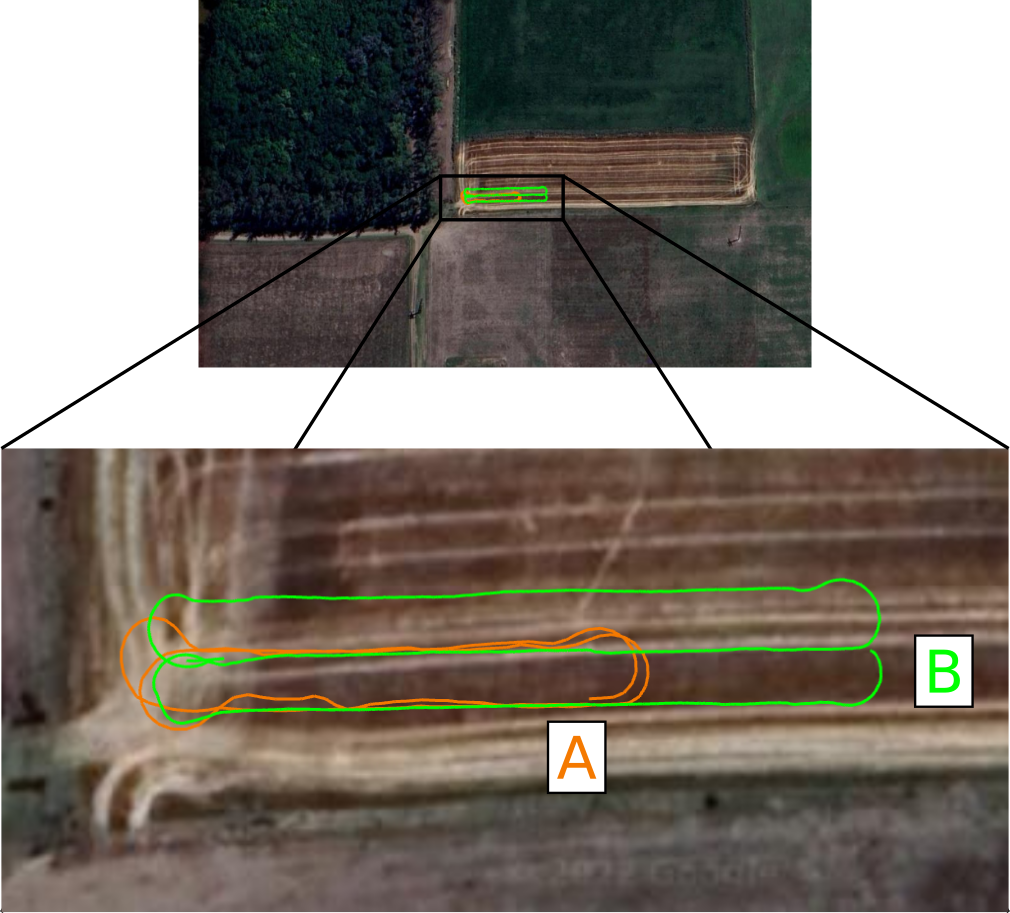
\includegraphics[width=\columnwidth]{images/satellital.png}
    \caption{GNSS-RTK trajectories for the sequences A (orange) and B (green) of the in-house recordings in the soybean field.}
    \label{fig:satellital}
\end{figure}

\begin{figure}[tp]
    \centering
    \subfloat{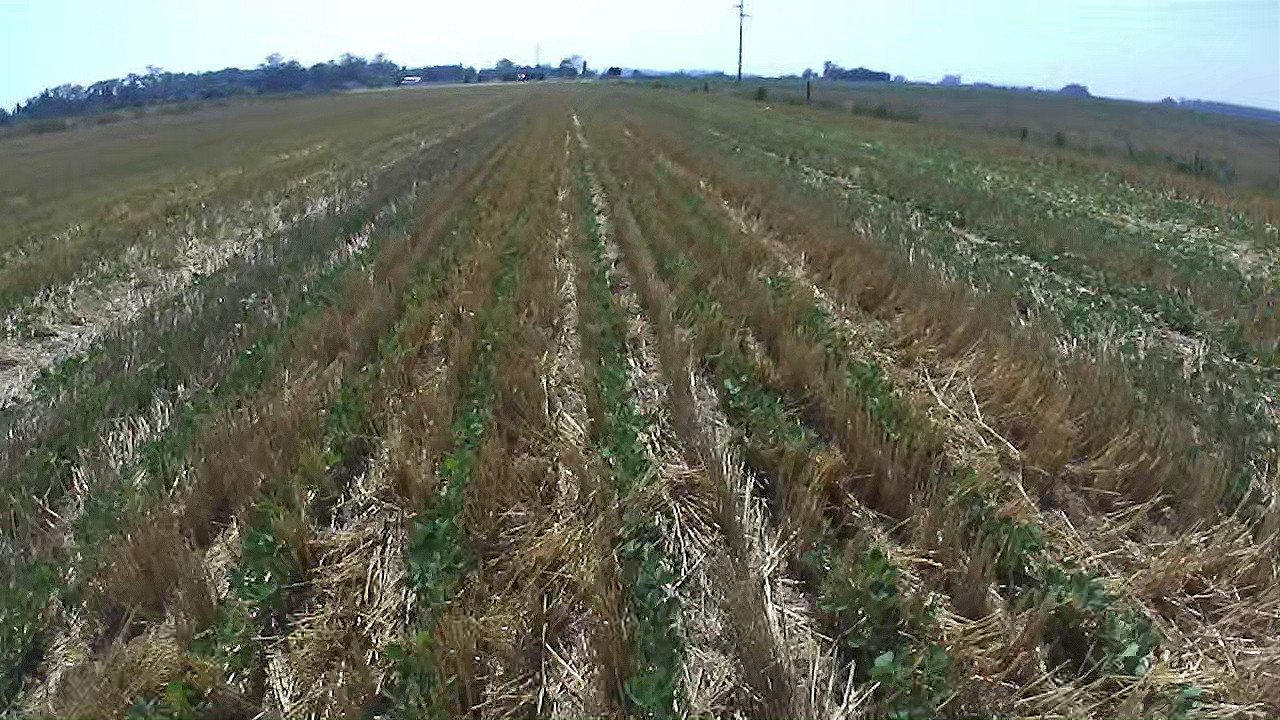
\includegraphics[width=0.45\columnwidth]{images/frame000000.jpg}}
    \hspace{0.1em}
    \subfloat{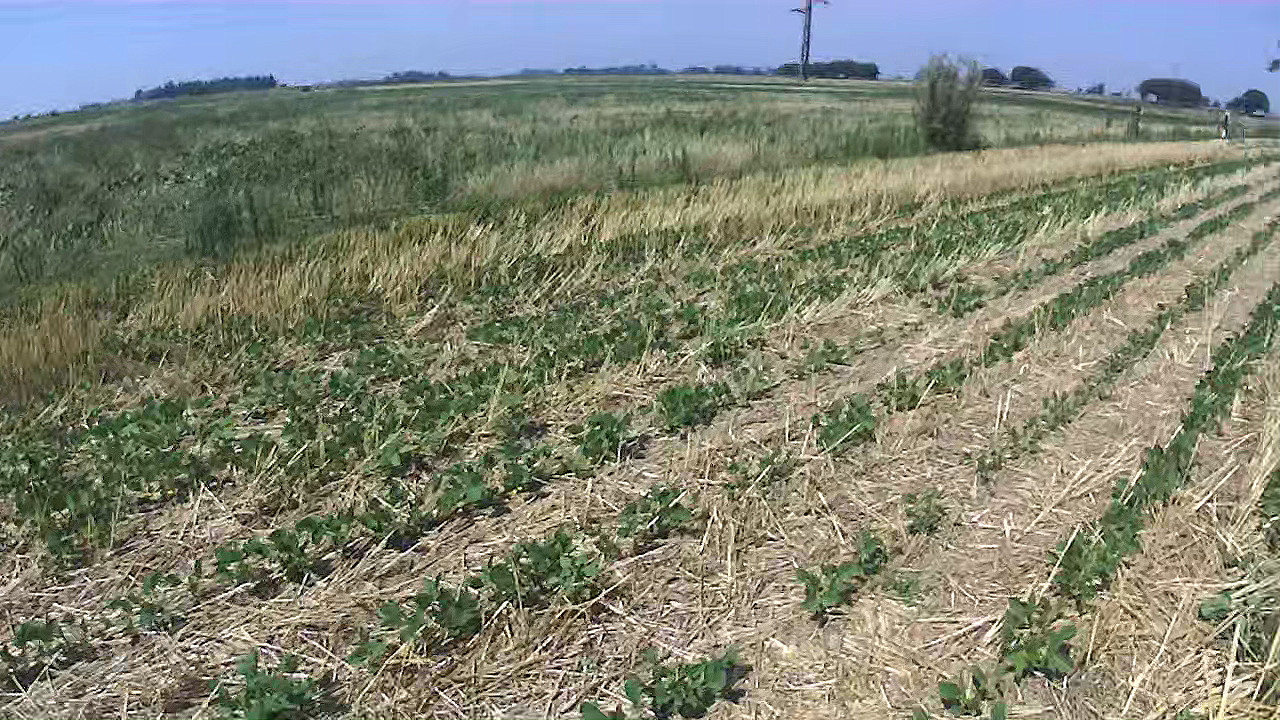
\includegraphics[width=0.45\columnwidth]{images/frame000136.jpg}}\\
    \subfloat{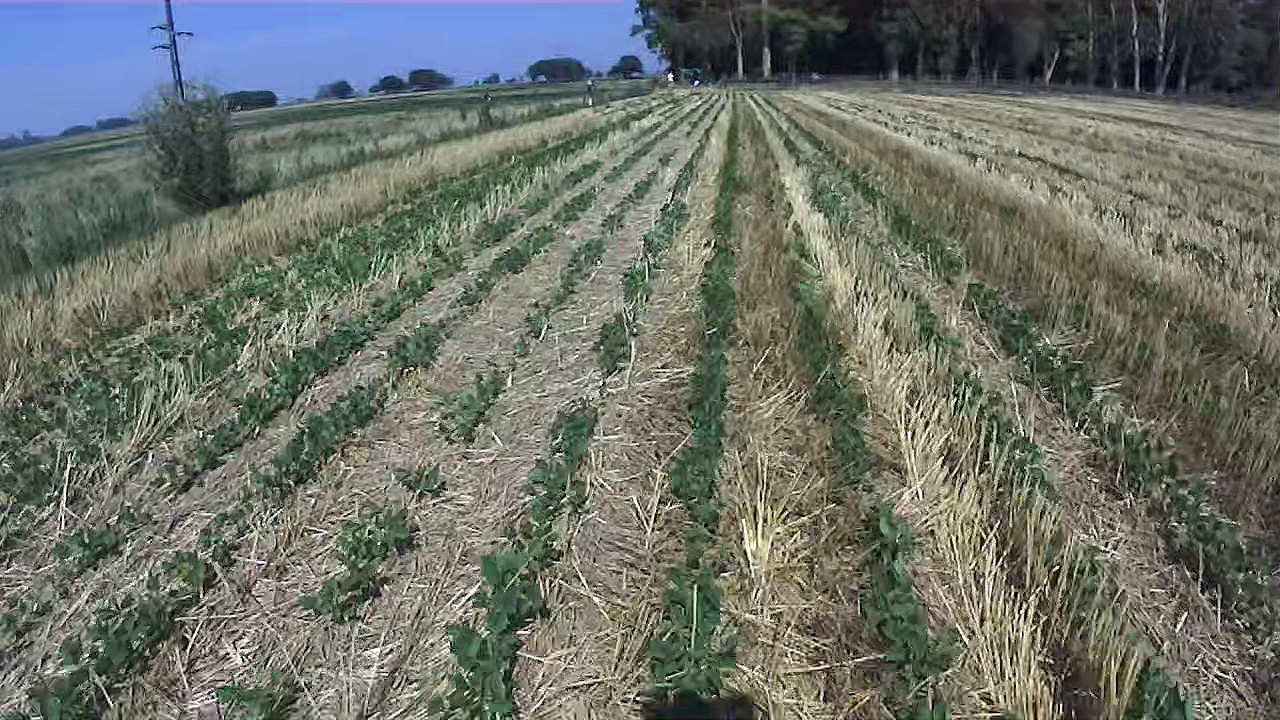
\includegraphics[width=0.45\columnwidth]{images/frame000200.jpg}}
    \hspace{0.1em}
    \subfloat{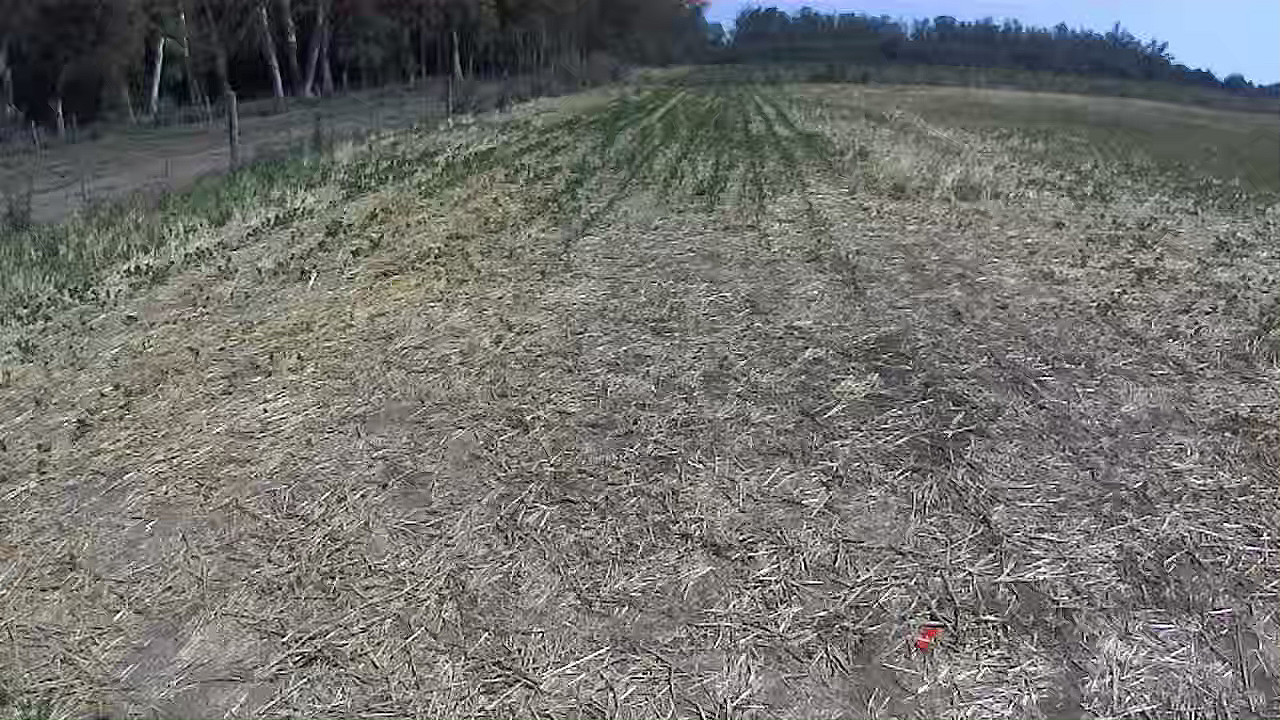
\includegraphics[width=0.45\columnwidth]{images/frame001264.jpg}}\\
    \subfloat{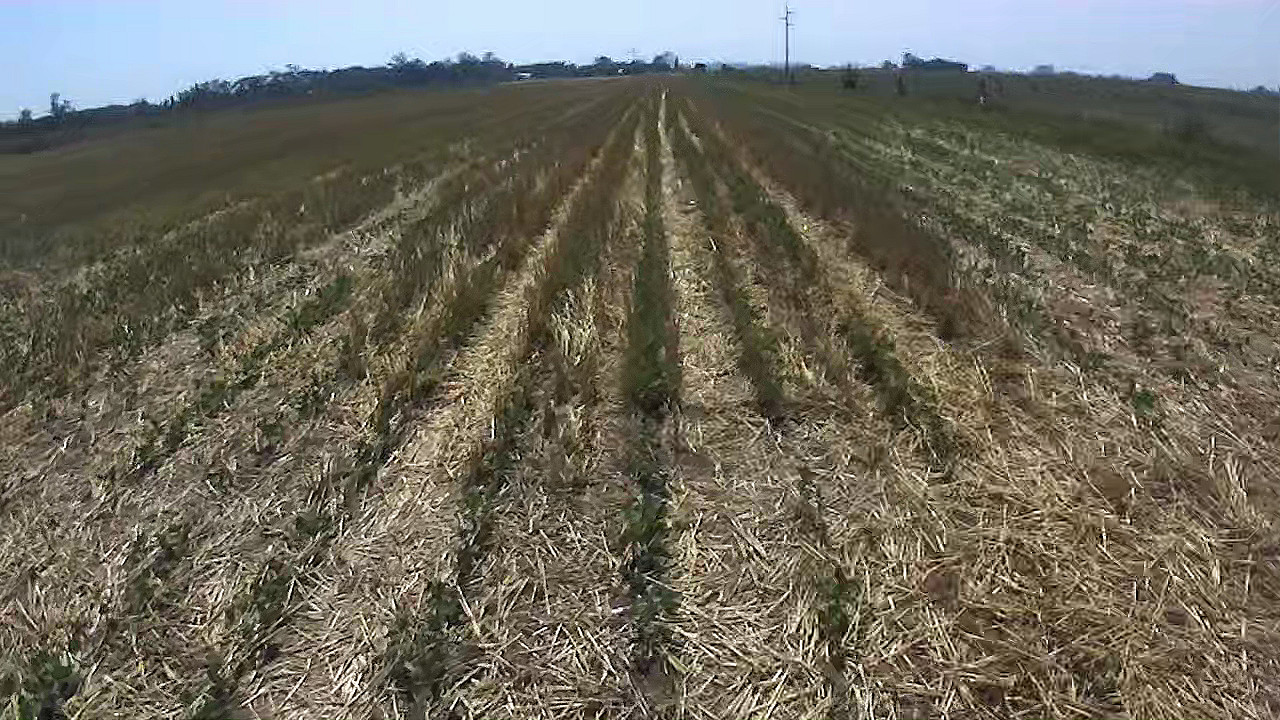
\includegraphics[width=0.45\columnwidth]{images/frame001364.jpg}}
    \hspace{0.1em}
    \subfloat{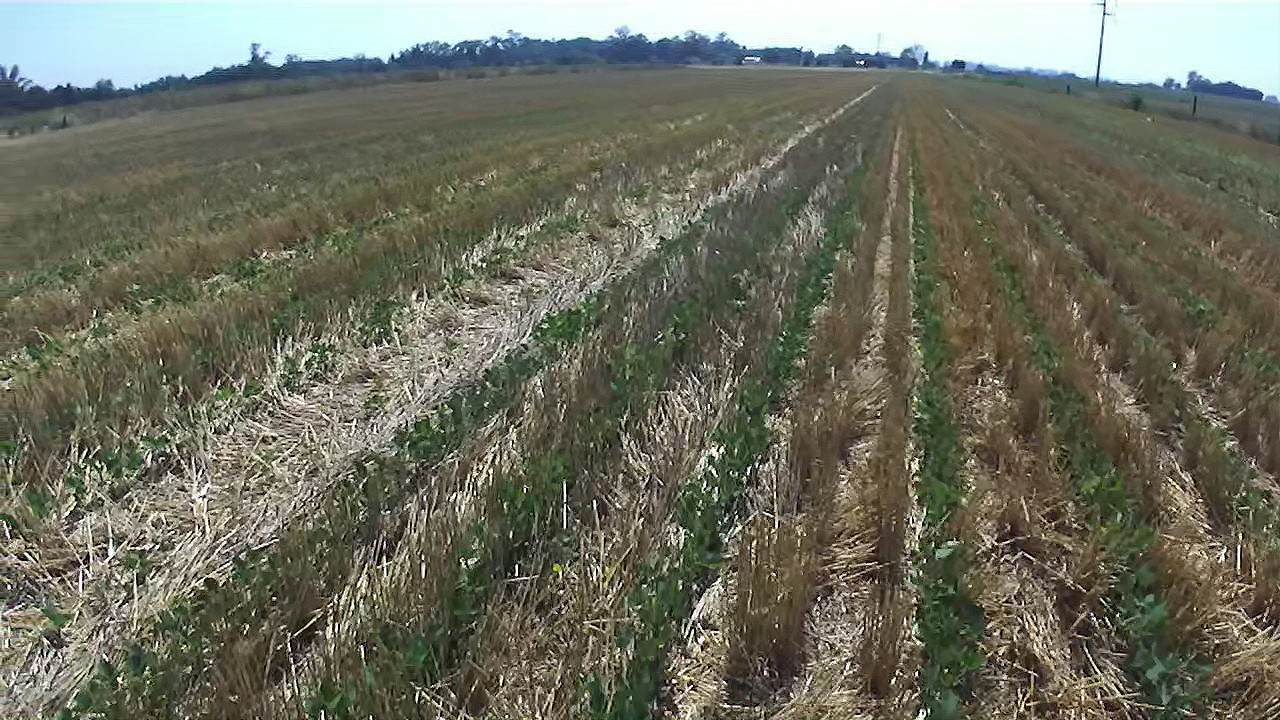
\includegraphics[width=0.45\columnwidth]{images/frame002477.jpg}}
    \caption{Sample images from our in-house dataset. Note the repetitive textures, a challenge for visual SLAM.}
    \label{fig:image_samples}
\end{figure}


On this data we ran the three frameworks mentioned in the previous experiment. The results of this experiment are shown in Table~\ref{tab:real_gps_results}, while the trajectories can be seen in the Figure~\ref{fig:trajectories_zavalla}. Estimated trajectories were aligned again with the ground-truth using
Umeyama's method.
\begin{table}[!tp]
    \centering
    \caption{Mean and standard deviation (between parentheses) of the Absolute Trajectory Error (ATE) [\si{\metre}] for stereo-inertial ORB-SLAM3 \cite{campos2021orbslam3}, a loosely-coupled GNSS-stereo-inertial system \cite{qin2019general} and our tightly-coupled GNSS-stereo-inertial framework in the in-house recordings in soybean fields. Best results are in \bf{bold}.}
    
    \resizebox{\linewidth}{!} {
        \begin{tabular}{cccc}
        \hline
                    Sequence & Stereo-Inertial & GNSS-Stereo-Inertial & GNSS-Stereo-Inertial \\
                    & \cite{campos2021orbslam3} & \cite{qin2019general} & (Ours) \\ \hline
        A &  0.64 (0.33) &  1.08 (0.78)                &  \bf{0.44 (0.16)} \\
        B & 0.43 (0.18)  &    5.58 (3.57)              & \bf{0.36 (0.13)} 
        \\
 \hline
        \end{tabular}
    }
    \label{tab:real_gps_results}
\end{table}

\begin{figure*}[!btp]
    \centering
    \subfloat[Sequence A\label{trajectories_sequence_A}]{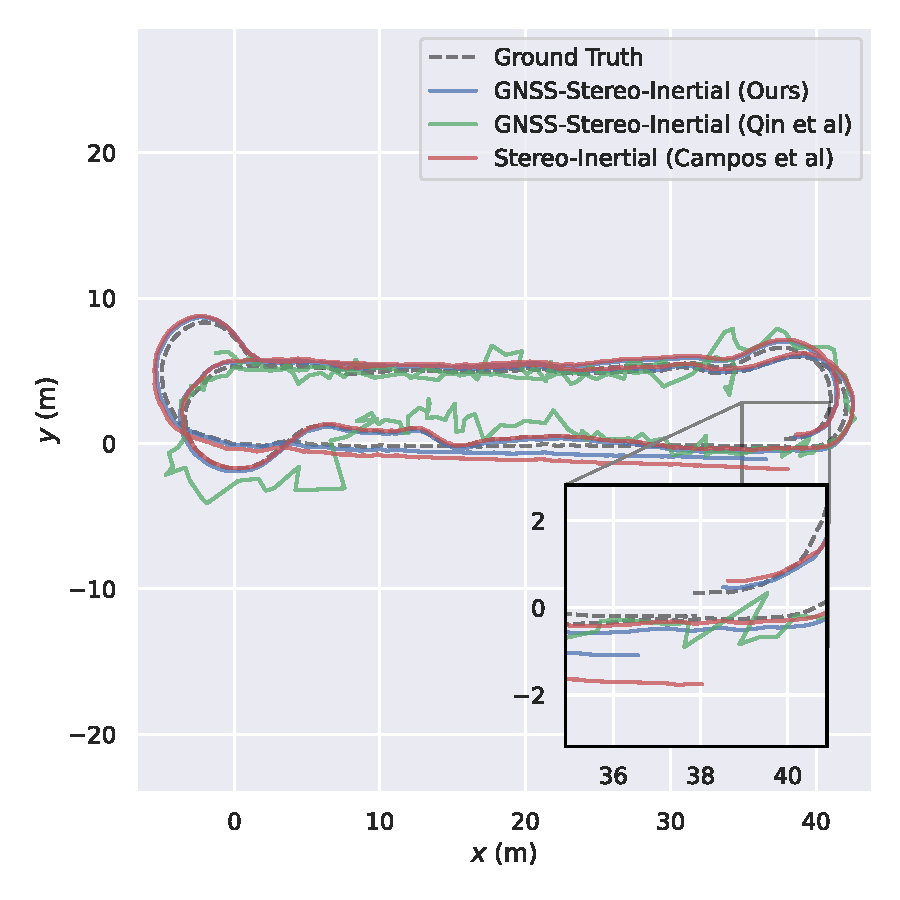
\includegraphics[width=0.42\textwidth]{images/zavalla_a.pdf}}
  \hspace{1cm}
  \subfloat[Sequence B\label{trajectories_sequence_B}]{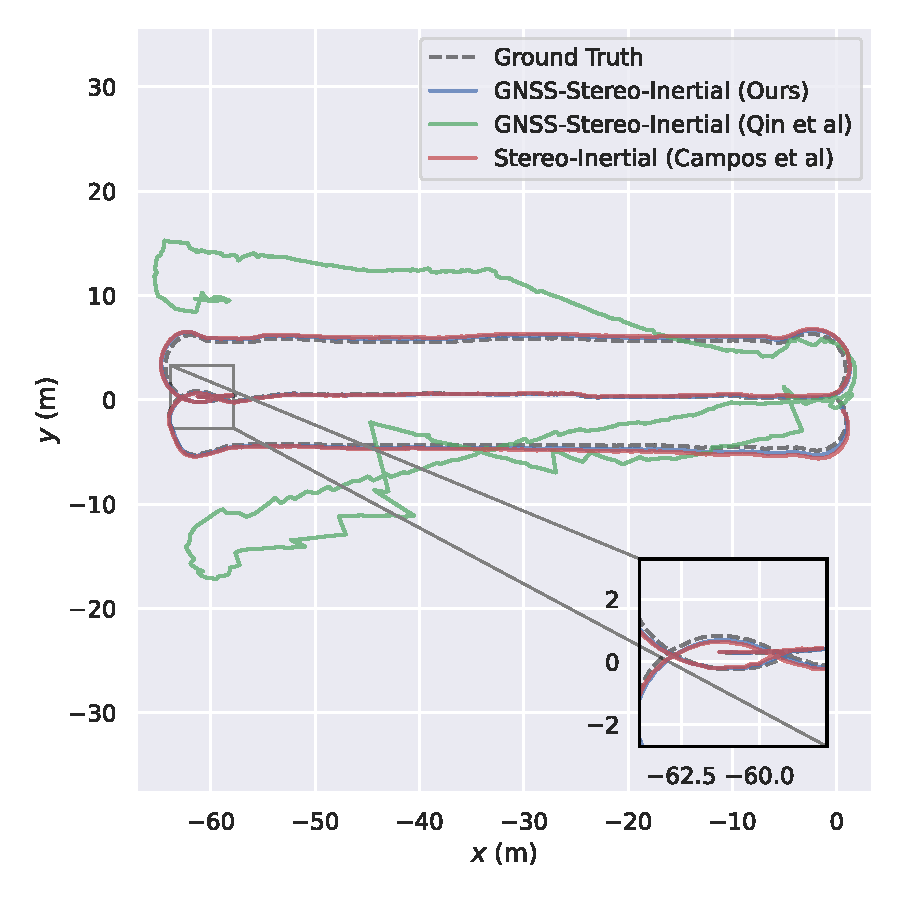
\includegraphics[width=0.42\textwidth]{images/zavalla_b.pdf}}\\
    \caption{Results from Stereo-Inertial ORB-SLAM3 \cite{campos2021orbslam3}, the loosely-coupled GNSS-Stereo-Inertial system of \cite{qin2019general} and our tightly-coupled GNSS-Stereo-Inertial implementation on our in-house recordings in soybean fields, using conventional GNSS. Note the smaller errors of tightly-coupled approaches, and how our GNSS fusion improves over the stereo-inertial baseline.}
    \label{fig:trajectories_zavalla}
\end{figure*}

\subsection{Discussion}
As can be seen in the results, our implementation clearly outperforms the stereo-inertial configuration of ORB-SLAM3 and the loosely-coupled approach in \cite{qin2019general}. As a very relevant note, we ran the full stereo-inertial ORB-SLAM3 in our configuration sequences with loop closure capabilities and, with its configuration by default, it was unable to detect previously visited locations and hence close loops due to insufficiently discriminative visual appearances of the agricultural environment (\emph{perceptual aliasing}). Although the default configuration for the loop closure parameters might be loosened to detect a higher number of loop closures, that would also produce a higher number of false positives (due again to perceptual aliasing) that would corrupt the estimation. These challenges are the main motivation for incorporating global positioning sensors in agricultural environments, allowing to reduce the drift without depending on visual features. Very interestingly, we found in our experiments that only one third of the optimized keyframes had associated GNSS measurements. This may indicate that high-frequency GNSS measurements are not necessary to improve the estimation of visual-inertial SLAM, and a sparse subset of them might suffice to offer a reasonable performance.

Unlike the loosely-coupled system, our implementation returns smoother trajectories. Moreover, since the fusion is loosely-coupled, the global position measurements correct the estimate without considering the continuous motion of the robot and acts as an interpolation between the underlying visual-inertial system and the GNSS measurement. Even though in sequence 02 of the Rosario Dataset, the loosely-coupled fusion system obtains a lower error, in the trajectory of the Figure~\ref{fig:trajectories_rosario} it can be observed that the estimation looks bumpy. Smooth pose estimation, like the one offered by our tightly-coupled approach, is more suitable for use in a navigation control algorithm.

Regarding the experiment with conventional GNSS measurements, it should be pointed out that the loosely-coupled system lost the visual-inertial tracking in the two sequences. This indicates that it is important not only to focus on global measurements, but also to have a robust visual-inertial fusion. In our case, we use ORB-SLAM3 as the underlying system, as a result of having analyzed the performance of different visual-inertial systems in previous research \cite{cremona2022evaluation}. As a conclusion, in addition to a tight coupling of the sensor data, the robustness of the visual-inertial estimates are also relevant for practical implementations in agricultural applications.

An important consideration is the modelling of the noise of GNSS measurements. Based on previous works \cite{cioffi2020tightly, boche2022dropout}, the uncertainty was modelled as additive isotropic Gaussian noise. This is a simple model that arises naturally from the GNSS device data, as the device drivers generally provide a covariance of the position. Other ways of modelling the noise of GNSS measurements in the context of pose estimation are worth studying, as when comparing the simulated signal in the section \ref{sec:experiments_rosario_dataset} experiment with the conventional GNSS signal used in the field experiments, differences in their behaviour were observed. When the conventional GNSS signal was inspected in detail, a bias was found, mainly at altitude, which could be verified by the GNSS-RTK. Therefore, this topic should be addressed in future work.
